\section{Технологический раздел}
В данном разделе предоставлено обоснование используемых языка программирования и среды разработки. Также приведены сведения о модулях и диаграмма классов приложения.

\subsection{Выбор и обоснование языка программирования и среды разработки}

При написании программного продукта был использован язык программирования Kotlin \cite{Kotlin}. 

Данный выбор обусловлен следующими факторами:
\begin{itemize}
\item задача подразумевает под собой разработку способа взаимодействия с базой данной InfluxDB с расширением функционала библиотеки The Kotlin InfluxDB 2.0 Client,
\item возможность запуска программного кода на любом устройстве, поддерживающем Java,
\item большое количество литературы, связанной с ЯП Java.
\end{itemize}

При разработке использовалась среда IntelliJ IDEA. Данный выбор обусловлен тем, что Kotlin является продуктом компании JetBrains, поставляющей данную среду.

\subsection{Сведения о модулях}
Приложение логически разделено на следующие части:
\begin{itemize}
\item модуль доступа к данным,
\item модуль бизнес-логики,
\item модуль реализации протокола,
\item модуль клиента,
\item модуль сервера.
\end{itemize}

Модуль доступа к данным включает в себя два класса, основанных на паттернах репозиторий (CharRepositoryImpl) и объекта доступа к данным (InfluxDAO). В данной реализации объект доступа к данным позволяет сделать репозиторий независимым от реализации исполнения запросов к базе данных. Данный объект использует InfluxDB-client-kotlin для запросов на внесение и чтение записей в базу данных, однако отдельный функционал (например, создание пользовательского хранилища) производится через HTTP-запросы напрямую к серверу InfluxDB с использование OkHttp3.

Модуль бизнес-логики включает в себя множество сущностей, фигурирующих между слоями клиент-серверной архитектуры.

Модуль реализации протокола включает в себя класс YDVP, который может представлять собой YDVP-запрос или YDVP-ответ, единственным различием для них будет интерпретация абстрактного класса StartingLine, от которого наследуются классы YdvpStartingLineRequest и YdvpStartingLineResponse. Данная часть также содержит класс YdvpParser, который предоставляет услуги парсинга приходящих YDVP-запросов.

Модуль клиента включает в себя класс InfluxServiceClient, который позволяет подключиться к удалённому серверу, отправлять на него YDVP-запросы и получать YDVP-ответы. 

Модуль сервера включает в себя всё необходимое для запуска сервера на заданном порту устройства.

\subsection{Структура и состав классов}

На рисунках \ref{fig:dataLayer} -- \ref{fig:serverAndProtocol} предоставлены диаграммы классов компонентов приложения.

\begin{figure}[H]
\begin{center}
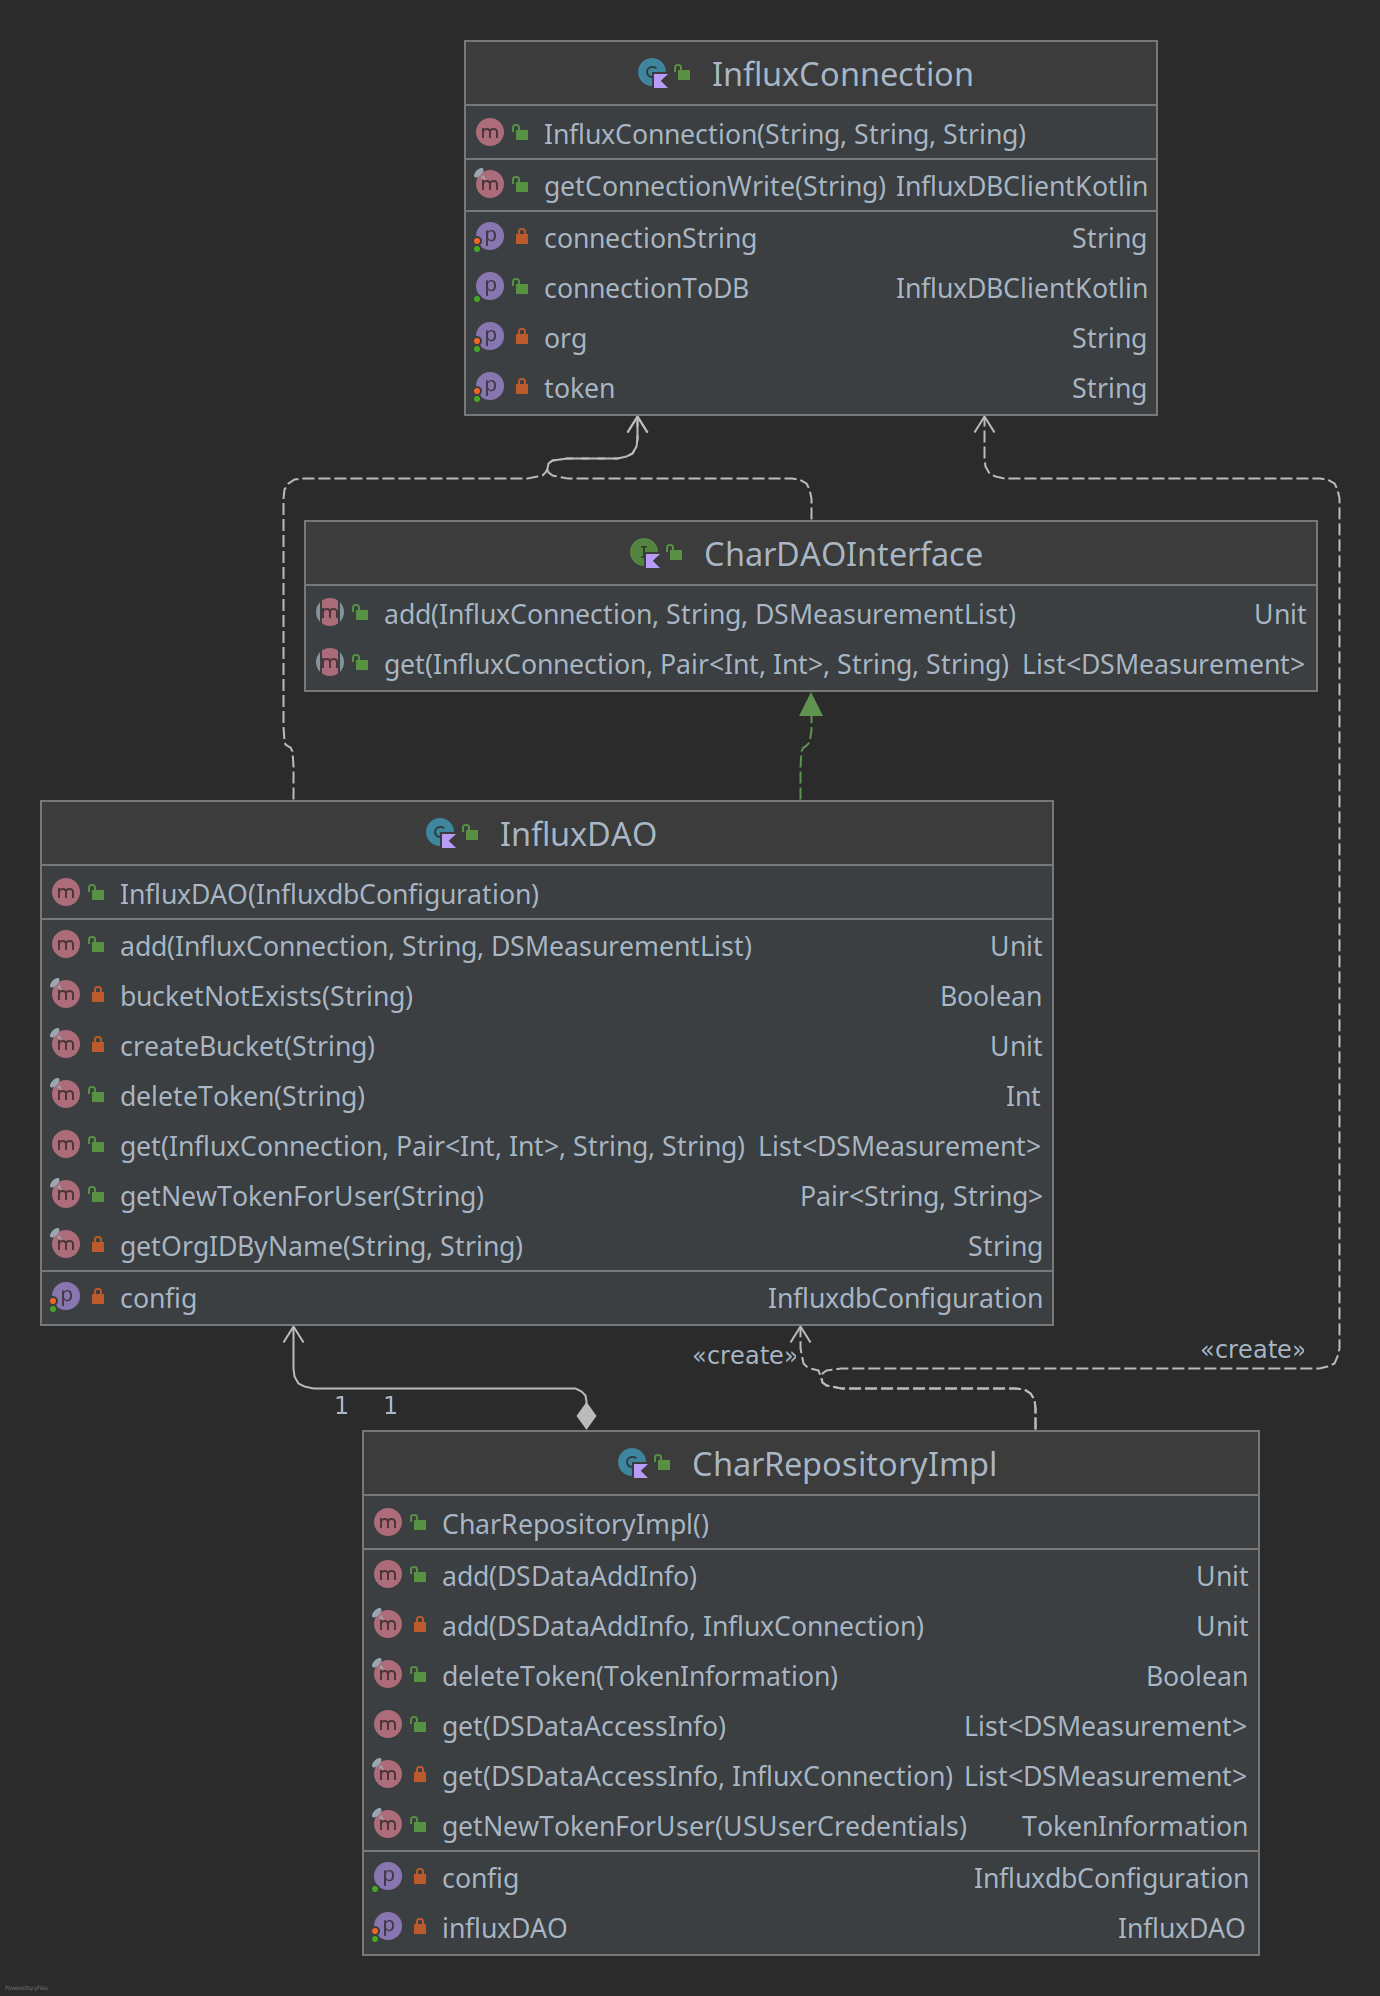
\includegraphics[width=\textwidth]{img/dataLayerDiagram.png}
\captionsetup{justification=centering}
	\caption{Диаграмма классов слоя доступа к данным приложения. }
	\label{fig:dataLayer}
\end{center}
\end{figure}

\begin{figure}[H]
	\centering
	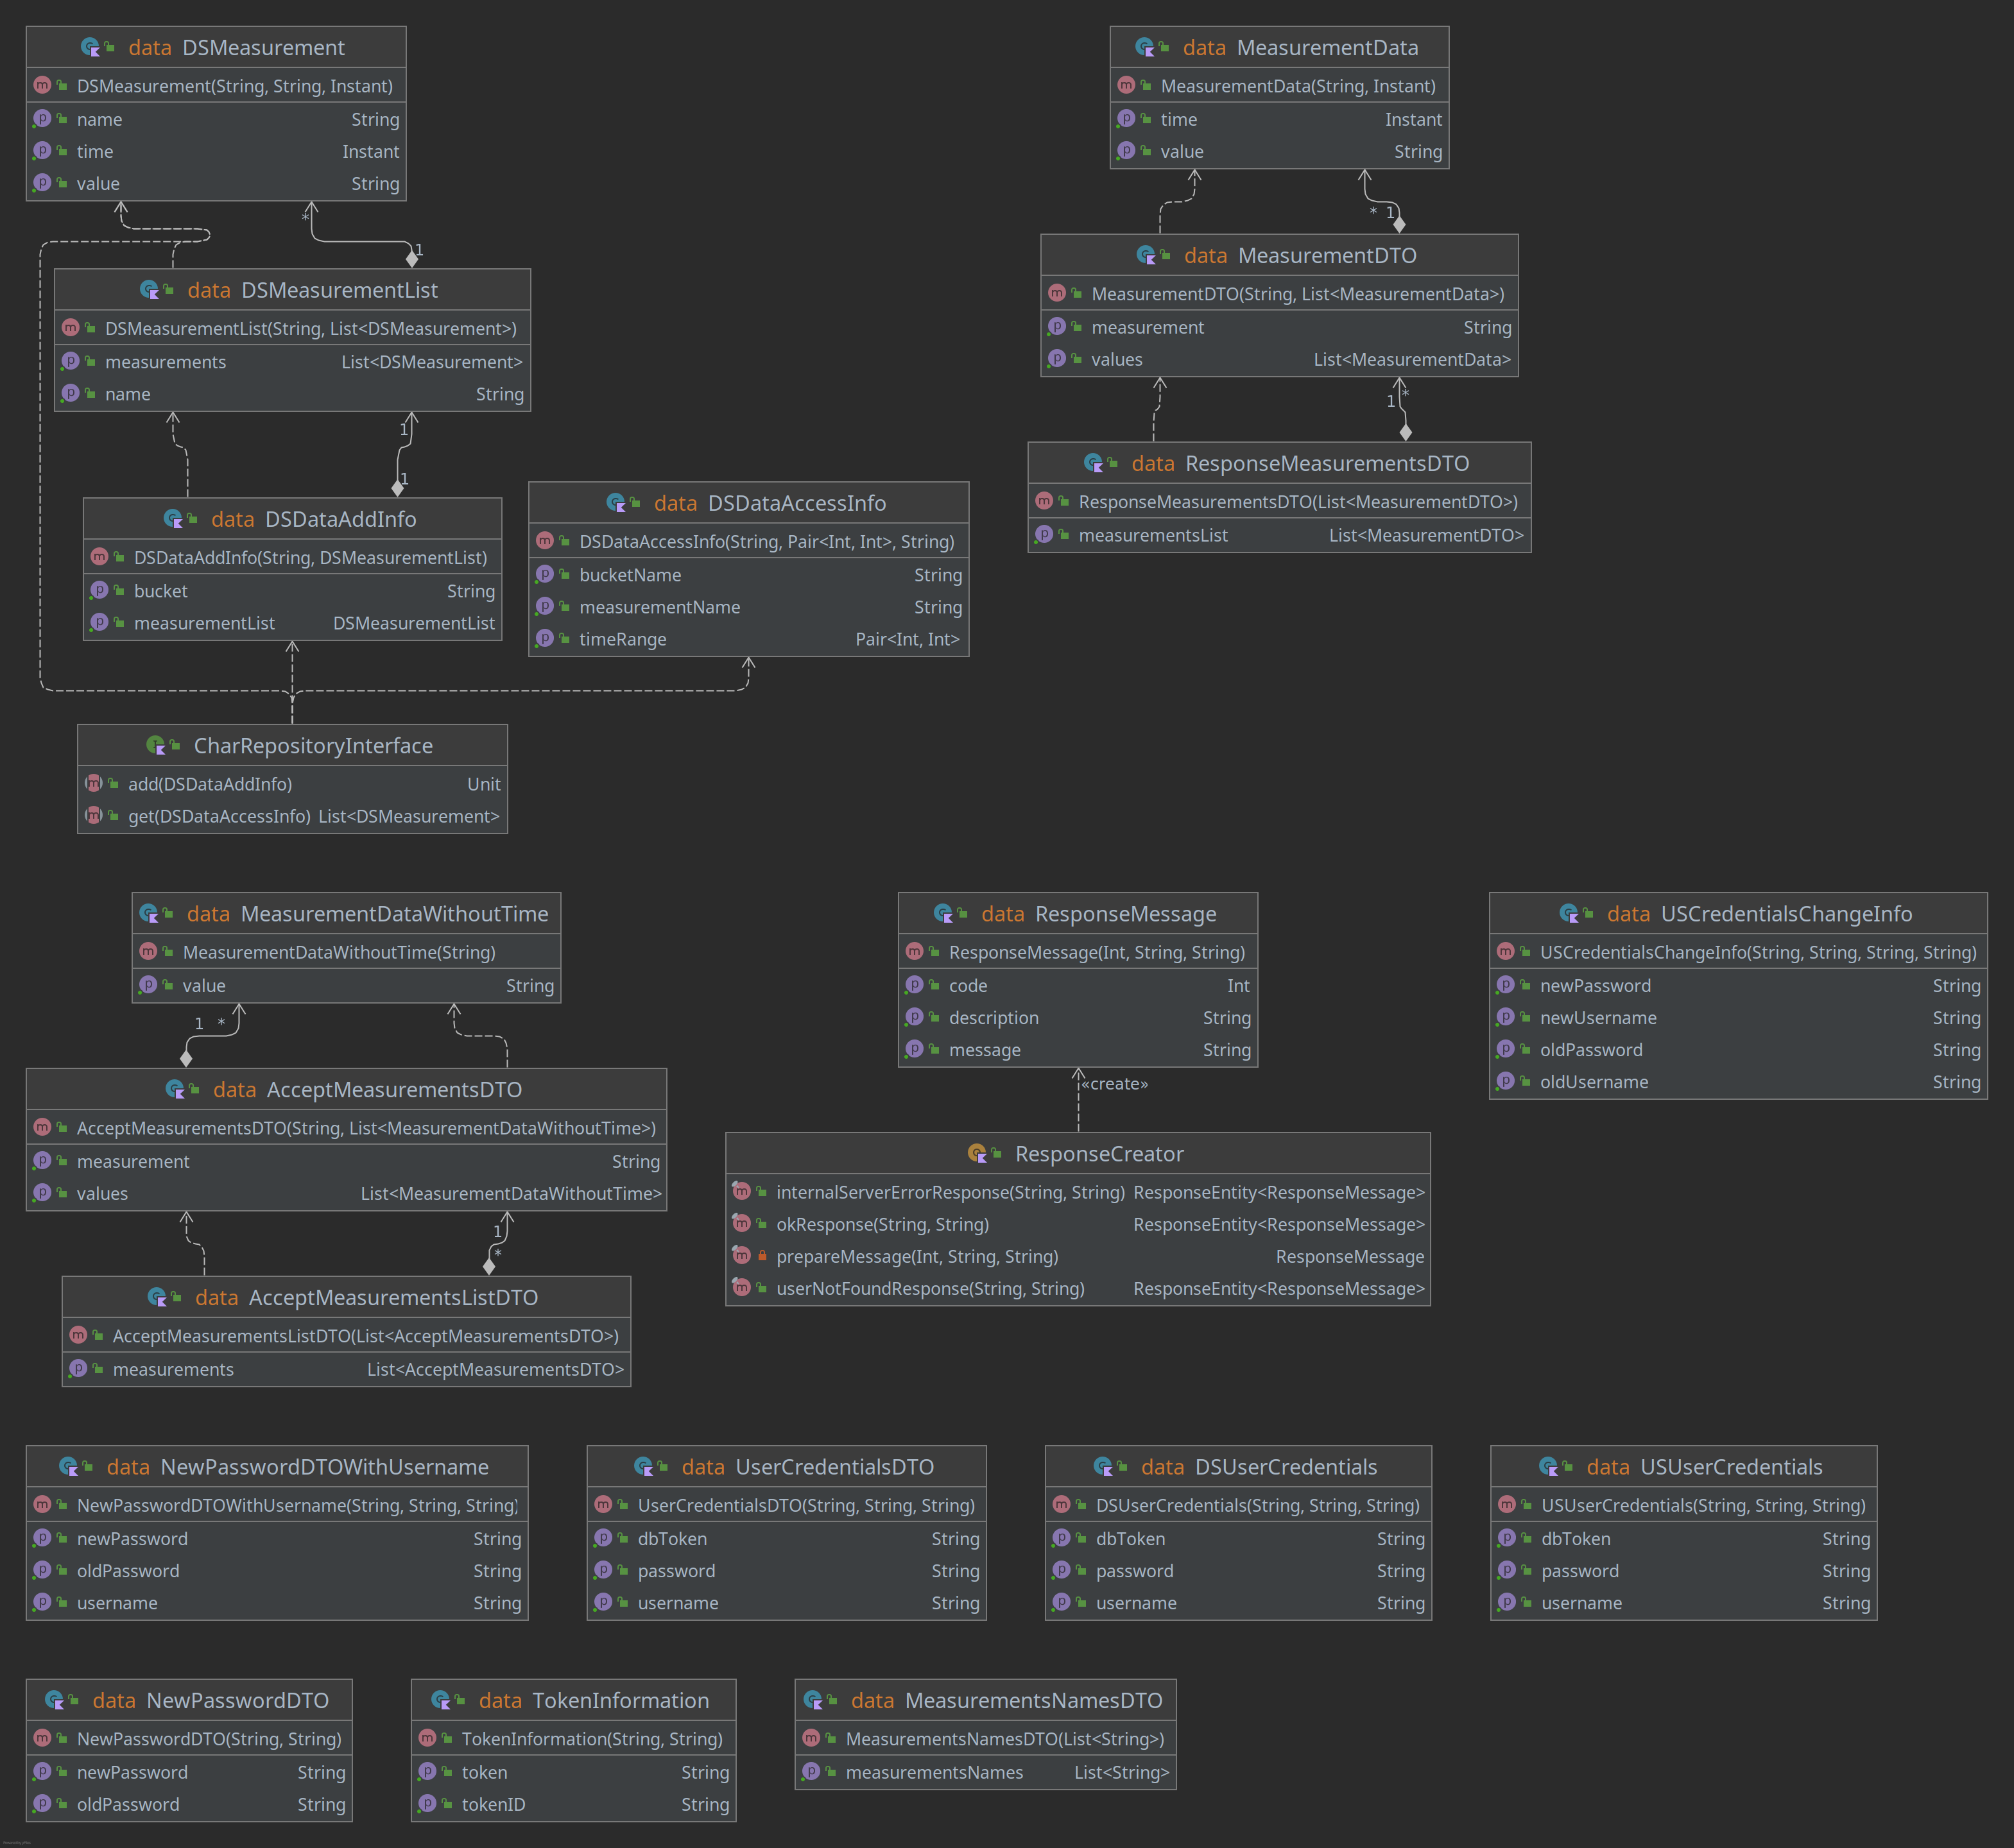
\includegraphics[width=\textwidth]{img/domainLayerDiagram.png}
	\caption{Диаграмма классов бизнес-логики приложения. }
	\label{fig:domainLayer}
\end{figure}

\begin{figure}[H]
	\centering
	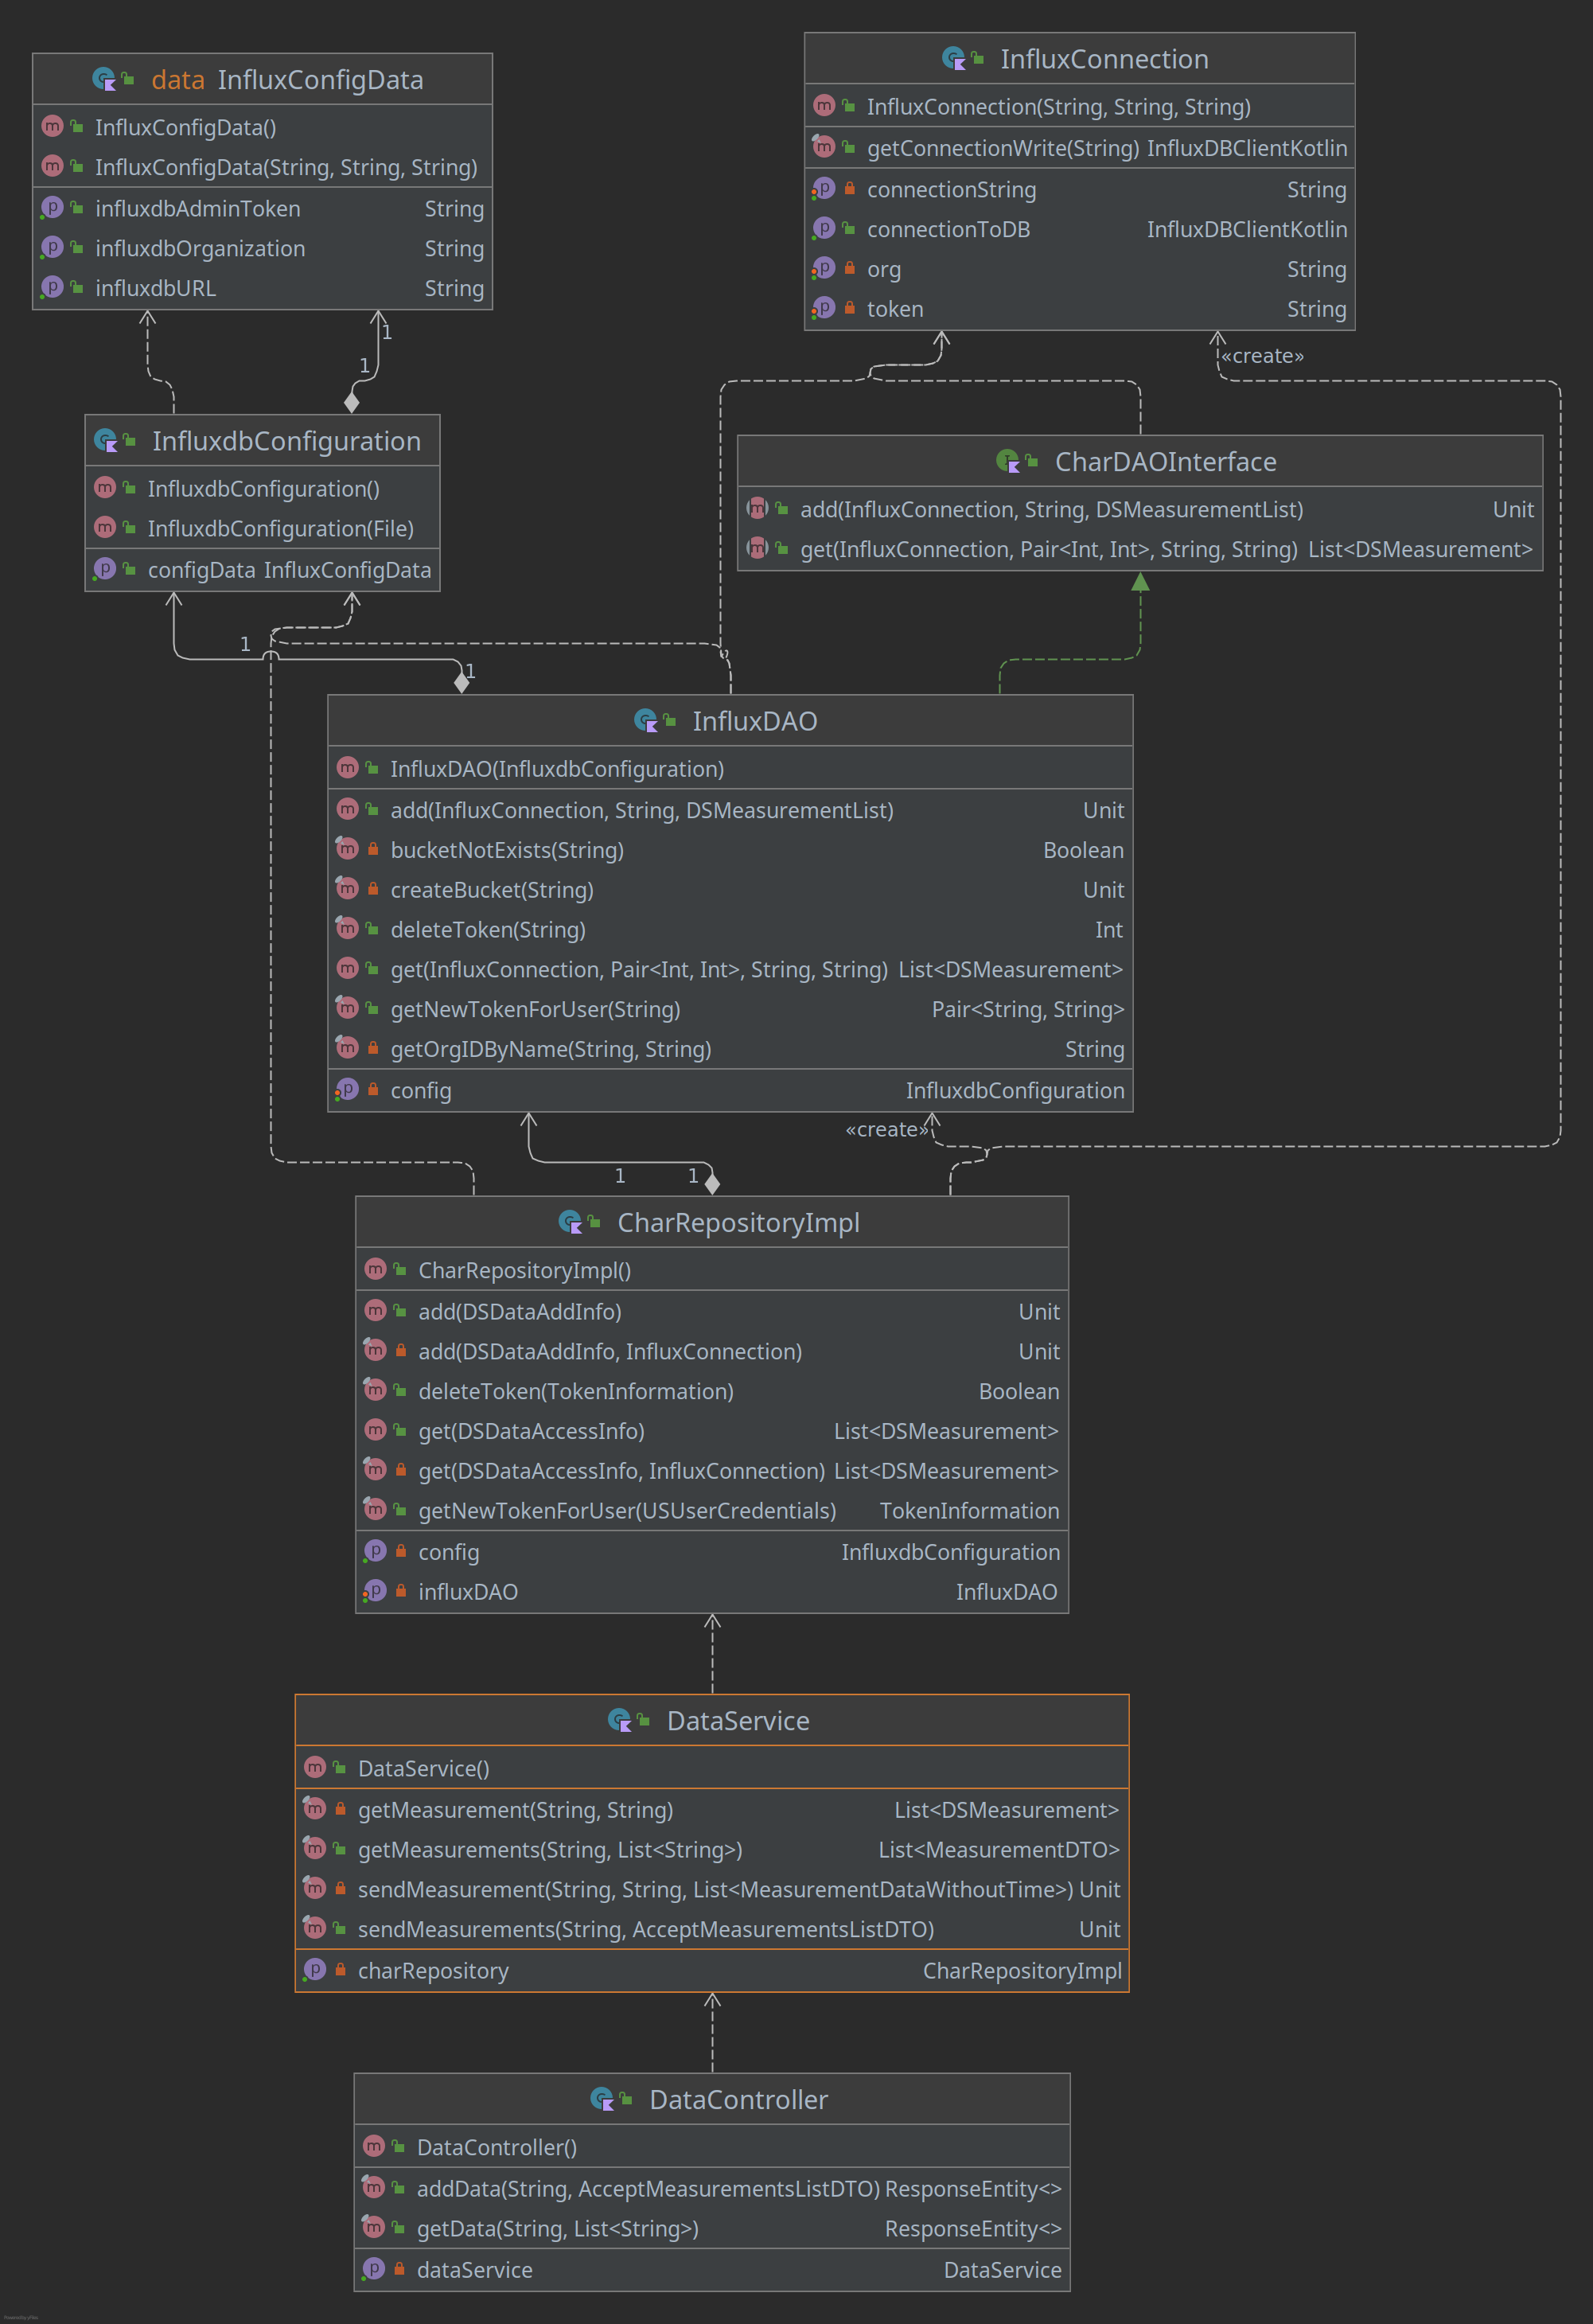
\includegraphics[width=\textwidth]{img/dataAndControllerLinkageDiagram.png}
	\caption{Диаграмма классов, показывающая связь контроллера и слоя доступа к данным. }
	\label{fig:dataAndController}
\end{figure}

\begin{figure}[H]
	\centering
	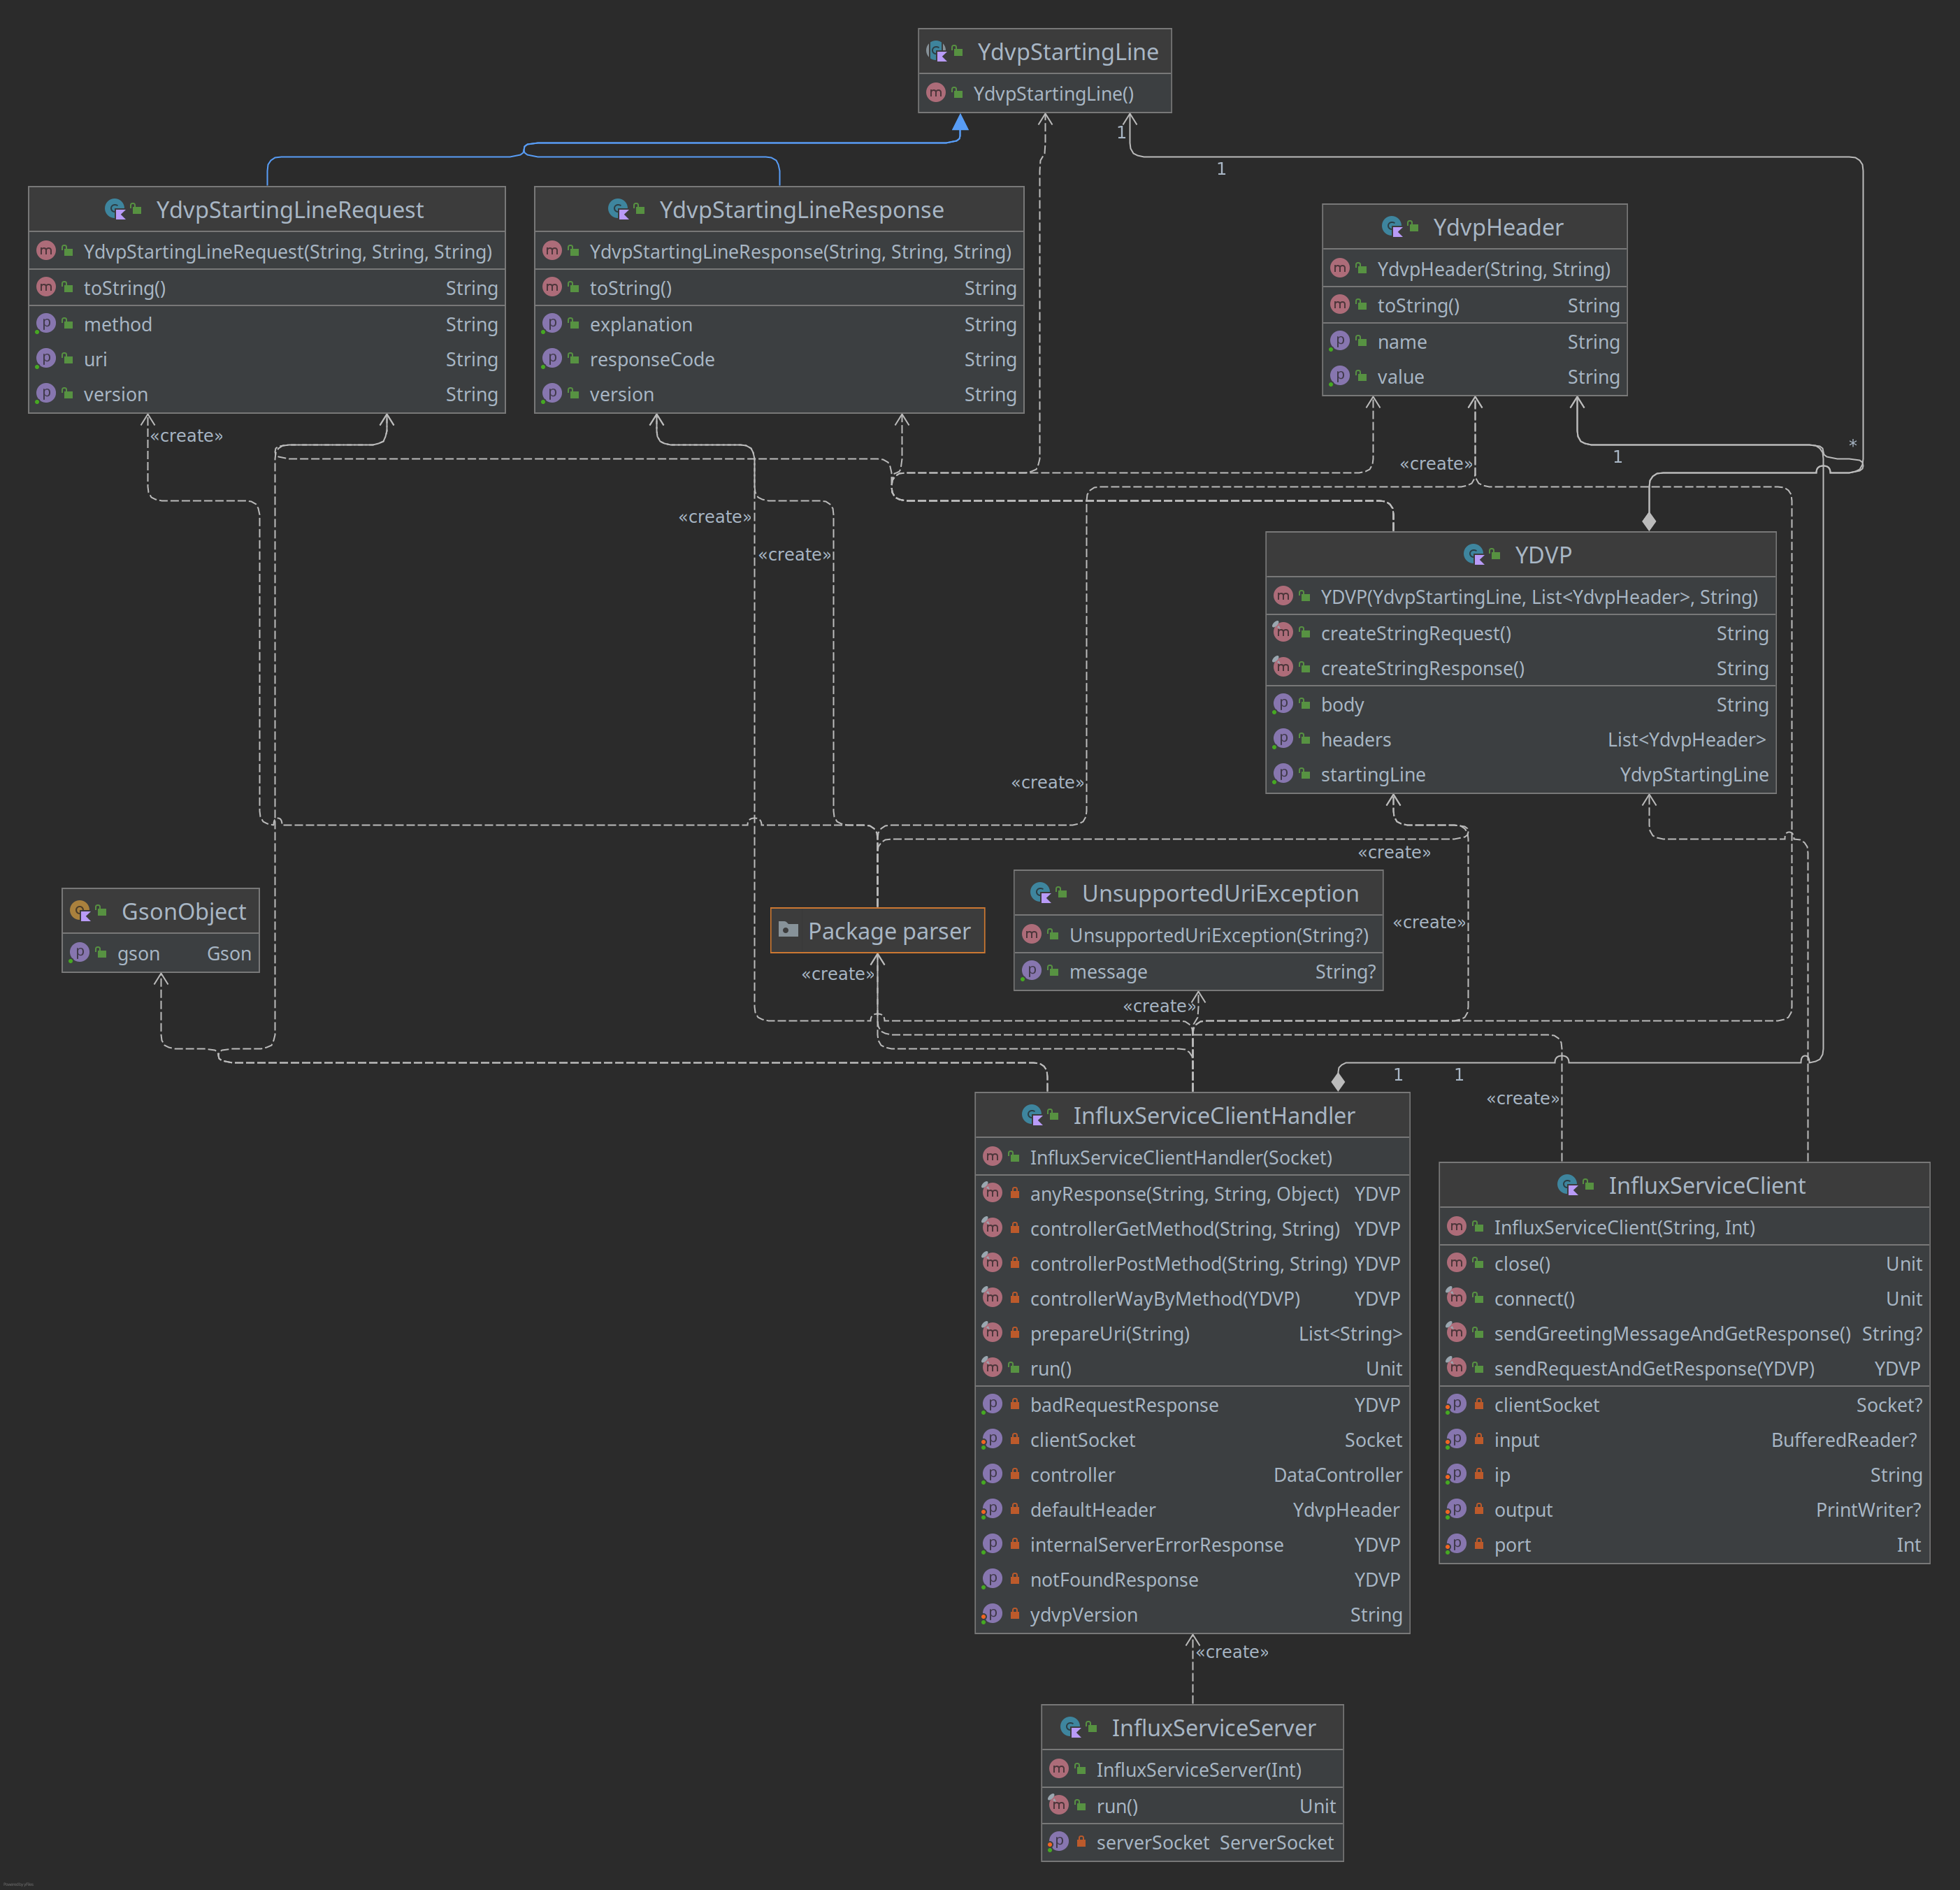
\includegraphics[width=\textwidth]{img/serverDiagram.png}
	\caption{Диаграмма классов серверной части приложения. }
	\label{fig:serverAndProtocol}
\end{figure}

\subsection{Пример использования приложения}

\subsection*{Вывод}
В качестве средств реализации были выбраны язык программирования Kotlin и среда разработки Intellij IDEA.

В разделе были предоставлены краткие сведения о модулях программы, в которых была предоставлена информация об используемых паттернах проектирования, а также системе взаимодействии классов в приложении.

Также были рассмотрены структура и состав классов, представленных в форме UML-диаграмм.